\documentclass{beamer} %
\usetheme{CambridgeUS}
%\usebeamercolor{lily}
\useoutertheme{infolines}
\usepackage{graphicx}
\usepackage{setspace}
\usepackage{tabularx}
\usepackage{tikzsymbols}
\usepackage{tikz}
\usepackage{spot}
\usepackage{tabularx}
\usepackage[absolute,overlay]{textpos}
\usepackage{booktabs}
\usepackage[backend=biber, style=authoryear]{biblatex}
\addbibresource{biblio.bib}


\newcommand\Factor{1.2}



\setbeamerfont{subtitle}{size=\large, series=\bfseries}
\definecolor{template}{RGB}{54, 114, 89}
\setbeamercolor{frametitle}{fg=template, bg=white}
\setbeamercolor{section in head/foot}{bg=template}
\setbeamercolor{subsection in head/foot}{bg=template!20, fg=template}
\setbeamercolor{author in head/foot}{bg=template}
\setbeamercolor{date in head/foot}{fg=template}
\setbeamercolor{title in head/foot}{fg=template}
\setbeamertemplate{frametitle}[default][center]

\definecolor{back}{RGB}{247, 251, 255}
\definecolor{map}{RGB}{111, 172, 232}
\definecolor{childmap}{RGB}{161, 200, 240}
\definecolor{nodemap}{RGB}{141, 170, 199}
\definecolor{rasch}{rgb}{0.0, 0.33, 0.71}
\definecolor{log}{rgb}{0.0, 0.65, 0.58}
\definecolor{diff}{RGB}{33, 113, 181}
\definecolor{single}{RGB}{106, 81, 163}
\definecolor{comp}{RGB}{35, 99, 70}
\definecolor{inc}{RGB}{191, 13, 43}
\definecolor{highlight}{rgb}{0.45, 0.31, 0.59}
\definecolor{section}{RGB}{51,51,179}
\definecolor{typical}{RGB}{8, 69, 148}
\definecolor{model}{RGB}{74, 20, 134}
\definecolor{orangered2}{RGB}{238,64,0}
\definecolor{royalblue3}{RGB}{58,95,205}
\definecolor{springgreen}{RGB}{0,205,102}
\definecolor{magenta}{RGB}{255,0,255}

  \tikzset{
	invisible/.style={opacity=0},
	visible on/.style={alt={#1{}{invisible}}},
	alt/.code args={<#1>#2#3}{%
		\alt<#1>{\pgfkeysalso{#2}}{\pgfkeysalso{#3}} % \pgfkeysalso doesn't change the path
	},
	every overlay node/.style={
		%draw=black,fill=white,rounded corners,
		anchor=north west, inner sep=0pt,
	},
}

\def\tikzoverlay{%
	\tikz[remember picture, overlay]\node[every overlay node]
}%



\title[Implicit assessment]{Implicit assessment in psychology: \\ How to work with implicit measures}

\date{June 9\textsuperscript{th}-10\textsuperscript{th} 2022}
\institute{University of Padova}
\author[Ottavia Epifania]{\texorpdfstring{Dr. Ottavia M. Epifania\newline\url{ottavia.epifania@unipd.it}}{Author}}

\usepackage{Sweave}
\begin{document}
	\tikzstyle{every picture}+=[remember picture]
\Sconcordance{concordance:seminario.tex:seminario.Rnw:%
1 74 1 1 0 228 1}


\begin{frame}
\maketitle
\end{frame}

\begin{frame}
	\tableofcontents
\end{frame}

\section{What we need}

\begin{frame}
	
	\begin{itemize}
		\item download \href{https://cran.r-project.org/bin/windows/base/}{
\includegraphics[width=0.04\linewidth]{R.png}} and follow the instructions
		\item download \href{https://www.rstudio.com/products/rstudio/download/}{
\includegraphics[width=0.10\linewidth]{Rstudio.png}} and follow the instructions
			\item Download \href{https://www.millisecond.com/download/}{
\includegraphics[width=0.10\linewidth]{inquisit.png}} and follow the instructions \textcolor{red}{!!! the demo version is valid only for a month!!} \href{https://www.rstudio.com/products/rstudio/download/}{
\includegraphics[width=0.10\linewidth]{Rstudio.png}} and follow the instructions 
			\item Download the \href{https://www.millisecond.com/download/library/iat/ageiat}{\textcolor{blue}{AGE IAT}} from Inquisit test library
		\item  \href{http://fisppa.psy.unipd.it/DscoreApp/}{
\includegraphics[width=0.10\linewidth]{AppLogo.png}} for analyzing the data (no need to install)
		
	\end{itemize}
\end{frame}

\section{The Inquisit file}
\begin{frame}
	\begin{enumerate}
		\item User manual (keep it or not)
		\item Labels and stimuli
		\item Instruction pages \& Performance summary
		\item Set up the experiment material
		\item Actual experiment
	\end{enumerate}
\end{frame}

\subsection*{Labels and stimuli}

\begin{frame}[fragile]
	Define ``Attribute A'' (in this case, ``\textcolor{green}{Good}'')
	
	\begin{columns}
		\begin{column}[T]{.50\linewidth}
				\begin{verbatim}
				<item attributeAlabel>
				/1 = "Good"
				</item>
				
				<item attributeA>
				/1 = "Joy"
				/2 = "Love"
				/3 = "Peace"
				/4 = "Wonderful"
				/5 = "Pleasure"
				/6 = "Glorious"
				/7 = "Laughter"
				/8 = "Happy"
				</item>
			\end{verbatim}
		\end{column}
	
		\begin{column}[T]{.50\linewidth}
			\vspace{5mm}
		First define the label of the evaluative dimension (i.e., ``Good'')
		
		\vspace{10mm}
		
		List all the attributes belonging to the superordinate category ``Good''
	\end{column}
	\end{columns}
	\vspace{5mm}
	So far, no details on the appearance of the text

\end{frame}

\begin{frame}[fragile]
	Same thing with the target category ``Target A'' (`in this case ``Young'' ), just remember to import the images (have to be in the same folder)
	
	\begin{columns}
		\begin{column}[T]{.50\linewidth}
			\begin{verbatim}
				<item targetAlabel>
				/1 = "Young"
				</item>
				
				<item targetA>
				/1 = "yf1.jpg"
				/2 = "yf4.jpg"
				/3 = "yf5.jpg"
				/4 = "ym2.jpg"
				/5 = "ym3.jpg"
				/6 = "ym5.jpg"
				</item>
			\end{verbatim}
		\end{column}
		
		\begin{column}[T]{.50\linewidth}
			\vspace{5mm}
			First define the label of the target category (i.e., ``Young'')
			
			\vspace{10mm}
			
			List all the elements belonging to the superordinate category ``Young'' (i.e., the images in the same folder)
		\end{column}
	\end{columns}
	
\end{frame}

\subsection*{Instruction pages \& Performance summary}

\begin{frame}[fragile]
		\begin{verbatim}
			<instruct>
			/ navigationbuttonfontstyle = 
			("Arial", 3%, false, false, false, false, 5, 1)
			</instruct>
		\end{verbatim}
	
	This defines the button to navigate through pages. Here you define its appearance, not its behavior. 
	
	To change the font:
	
	\begin{verbatim}
		("font-name", height, bold, italic, underline, strikeout, 
		quality, set)
	\end{verbatim}

font-name: e.g., ``Arial'', ``Tahoma'', ``Courier New''

quality: quality of the font, 1-5

set: characters set (e.g., latin, greek. 1 stands for the default of the computer on which Inquisit runs)
	\end{frame}

\begin{frame}[fragile]
	
	\begin{verbatim}
		
	<item instructions>
	/ 1 = "Put your left[...]."
	
	/ 2 = "Put your left finger [...]"
	
	/ 3 = "Press the left 'E' "
	
	[...]
	</item>
\end{verbatim}

\vspace{5mm}
Same as the attribute stimuli ``Good'', here the instructions are defined as a list of items

Again, this is only the content of the instructions

\end{frame}

\begin{frame}[fragile]
	\begin{verbatim}
		'<%item.attributeAlabel.item(1)%>' 
	\end{verbatim}

Allows for automatically including the label of attribute A in the instruction text. It uses ``item'' because it is supposed to be ``fixed''

\begin{verbatim}
	'<%expressions.leftTarget%>'
\end{verbatim}

Allows for automatically including the target \textbf{displayed on the left side of the screen}. It uses ``expressions'' because the target displayed on the left side of the screen changes according to the experiment 

\end{frame}


\begin{frame}[fragile]
\begin{figure}
	\centering
	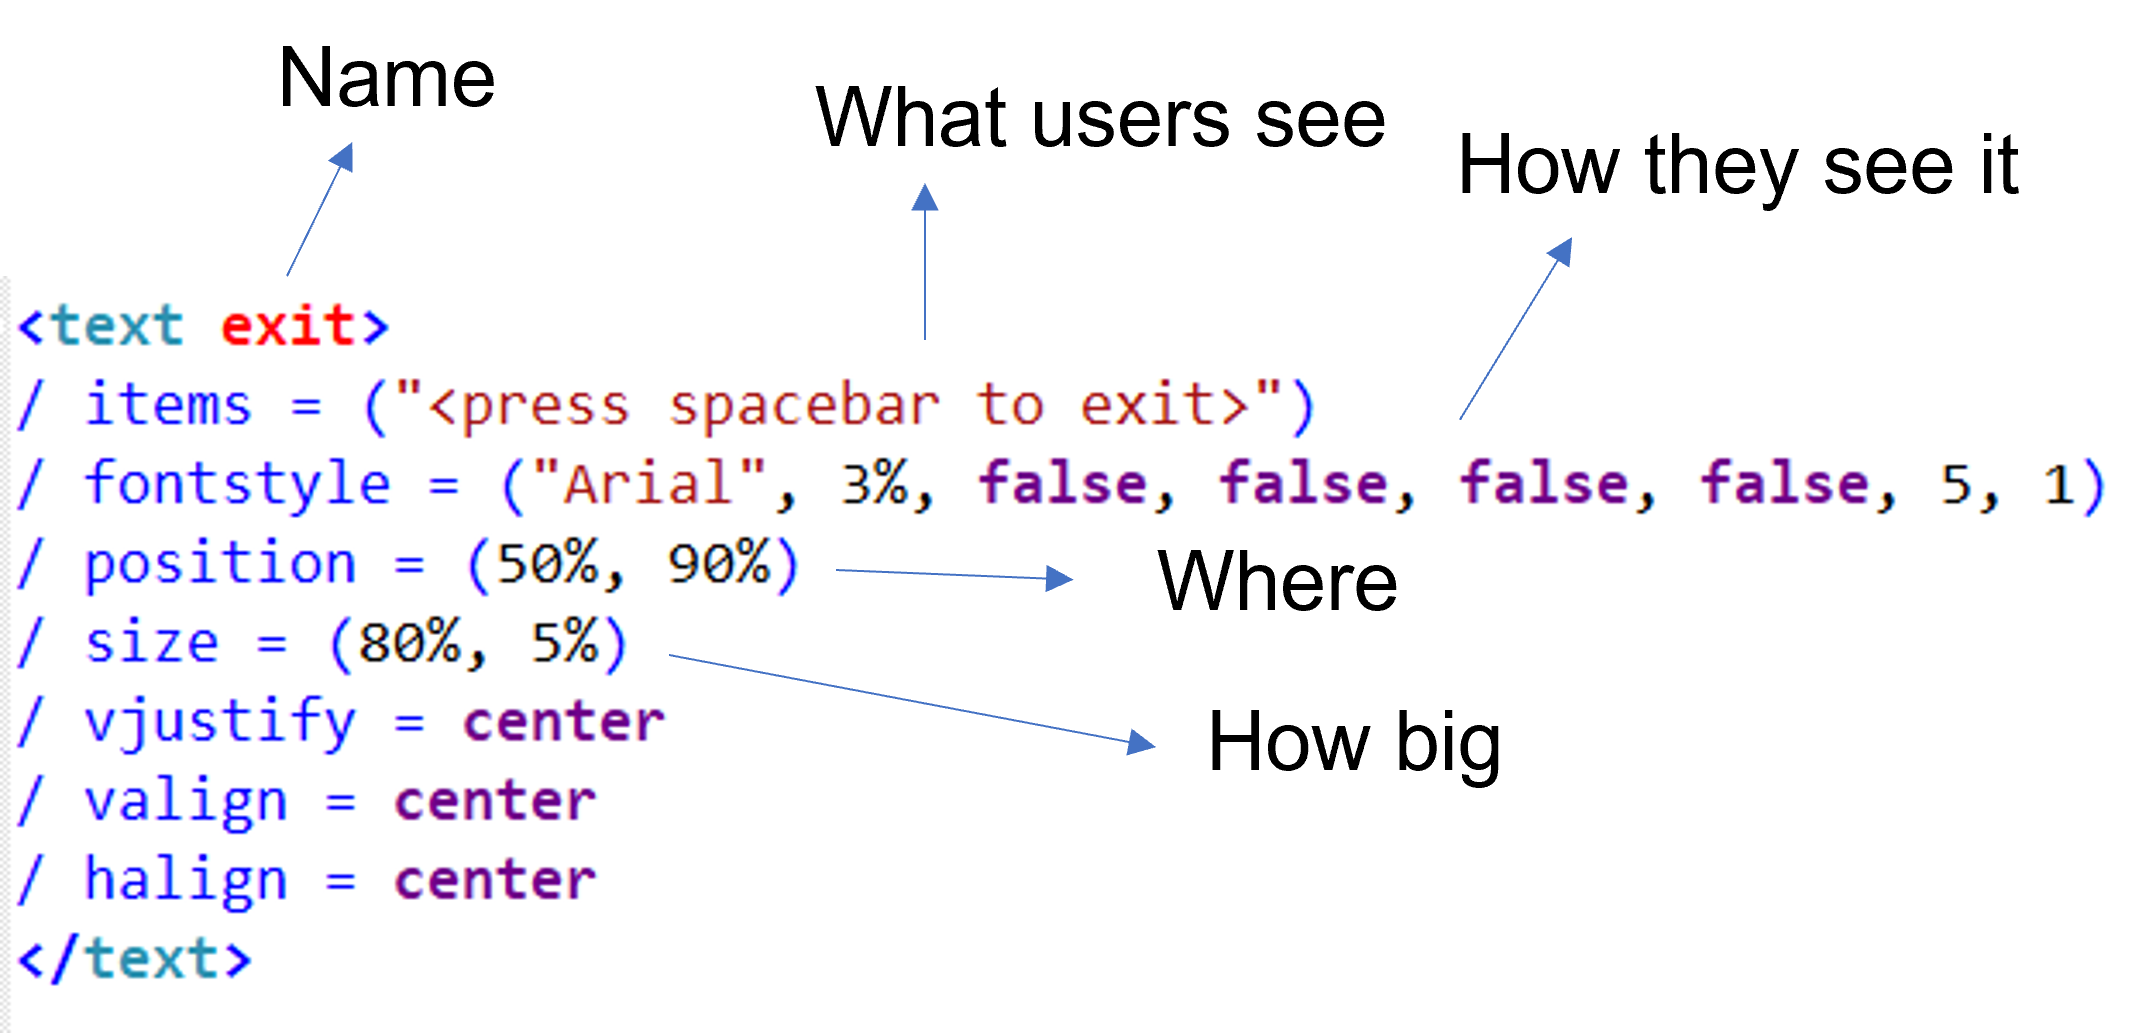
\includegraphics[width=.80\linewidth]{textThank.png}
\end{figure}

\vspace{3mm}
No actual behavior has been defined yet
\end{frame}

\subsection*{Set up the experiment material}
\begin{frame}[fragile]
	Use what defined in \texttt{<item instructions>} (\texttt{/items = instructions}) and add some fancy formatting: 
	
	\begin{verbatim}
		<text instructions>
		/ items = instructions
		/ position = (10%, 25%)
		/ halign = left
		/ valign = top
		/ hjustify = left
		/ vjustify = center
		/ size = (80%, 50%)
		/ select = values.instructionIndex
		</text>
	\end{verbatim}

\texttt{/ select = values.instructionIndex} tells which page of instructions to show

\end{frame}

\begin{frame}[fragile]
	With ``<trial instructions>'' we finally set the behavior of ``instructions'' throughout the experiment: 
	
	\begin{verbatim}
		<trial instructions>
		/ ontrialbegin = [
		values.progresswidth += 10;
		values.instructionIndex += 1;
		]
		/ stimulustimes = [1=instructions, spacebar, progressbar, progressbar_fill]
		/ correctresponse = (" ")
		/ errormessage = false
		/ recorddata = false
		/ showmousecursor = true
		</trial>
	\end{verbatim}

\texttt{/ stimulustimes = [1=instructions, spacebar, progressbar, progressbar\_fill]} tells the stimuli that have to be included in the \texttt{instructions} trial.

\end{frame}

\section{Data analysis!}


\end{document}
